\chapter{Research Design}
\label{ch:researchDesign}
All of our research methods are of a qualitative nature meaning no empirical data is collected. This Chapter provides an overview of our chose research methods, how they attempt to answer the research questions and discusses why these methods were chosen.

\section{Overall plan}
\label{sec:overview}
This section provides an overview of how our chosen research methods relate to each other and how they assist in answering the research questions we have posed. Table~\ref{tab:designPlan} gives a quick overview of our methods and which specific research question the method contributes to. The table order corresponds to when in our project the research method was used.

The first research question is concerned with finding relevant scenarios for the use of systems such as the one we are creating. To answer this question we preformed interviews and focus groups. A large part of the second focus group was dedicated to discussing different scenarios with the physiotherapists.

The second research question asks what functional and user experience requirements the visualizations should have. The initial requirements were gathered through an interview with a domain expert. Two additional revisions of the requirements were planned, one after each focus group. Feedback on the prototype was the basis for the modifications to the requirements. A portion of the second focus group was used to discuss the requirements with the physiotherapists.

Research question 3 asks which visualizations the physiotherapists prefer, given the requirements and scenarios created. Feedback on the visualizations was given in the focus groups. The larger part of both focus groups was dedicated to discussing and reviewing the visualizations with the physiotherapists. 

\begin{table}[h!]
  \centering
  \begin{tabular}{|p{0.7cm}|p{2.2cm}|p{8.8cm}|}
    \hline
    \textbf{RQ} & \textbf{Method} & \textbf{Description} \\ \hline
    1,2 & Interview & An interview was performed with a domain expert to establish initial requirements and scenarios. \\ \hline
    2 & Brainstorming & Based on the initial requirements, the authors performed brainstorming sessions among themselves and sketches were created. \\ \hline
    2, 3 & Prototype & The paper sketches were used as a starting point to create a high fidelity prototype that would be presented to the first focus group. \\ \hline
    1,2,3 & Focus group & The first running prototype was presented to the focus group and would enable us to refine it further. \\ \hline
    2, 3 & Prototype & Based on the feedback received from the first focus group the prototype was modified and improved. \\ \hline
    None & Questionnaire & Before the final focus group, a quick questionnaire was answered by the users. \\ \hline
    1,2,3 & Focus Group & The new version of the prototype was presented and the requirements were refined. \\ \hline
    1,2 & Interview & The interview was carried out to help us understand how the physiotherapists work. \\ \hline
  \end{tabular}
  \caption{The overall design plan.}
  \label{tab:designPlan}
\end{table}

More detailed information about how the methods were executed and their result can be found in the subsequent chapters of this report, namely in Chapters 6 to 10. The following sections of this chapter explain the rationale and choice of method in further detail.
 
\section{Overall plan in accordance to ISO}
This section aims to show how our chosen research methods relate to human-centred design activities describes in ISO 9241-210. Figure~\ref{fig:hcdActivitiesOurs} show how our research methods correspond to the ISO activities. The gray text is the purpose of the step described in ISO 9241-210, inside of the squares are our research methods with a numbering showing the order in which they were executed. The brainstorming and questionnaire activities have been omitted from the figure, as they were primarily used as support methods for prototype 1 and focus group 2.

\begin{figure}[h!]
	\centering
		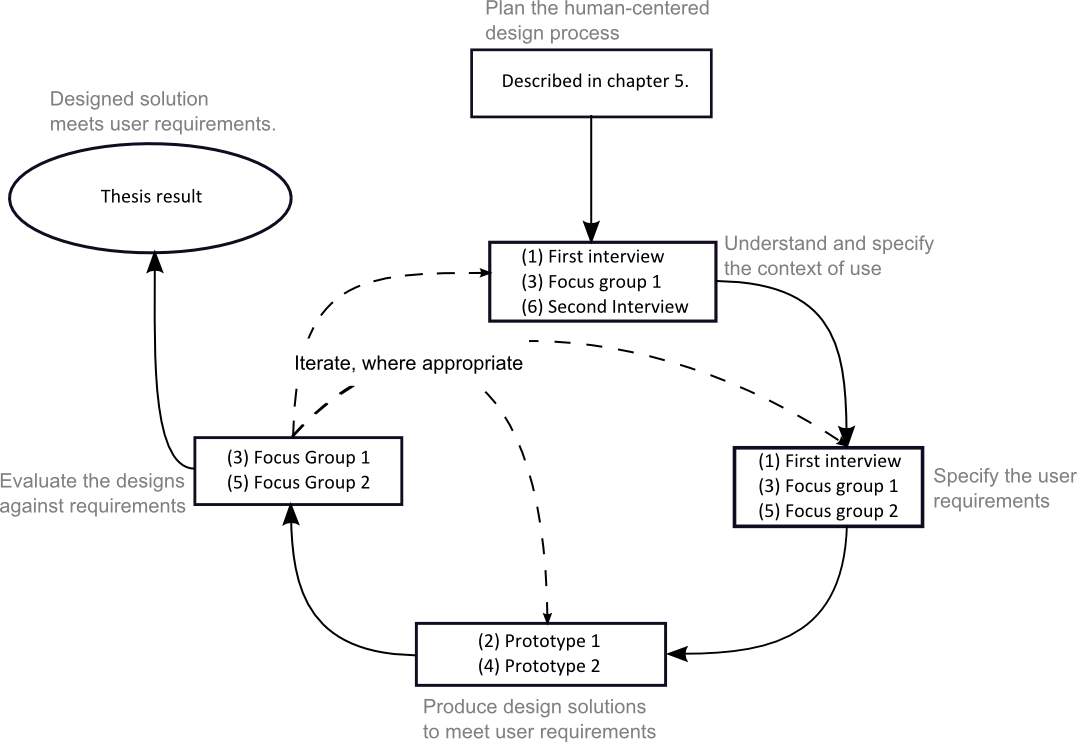
\includegraphics[width=0.9\textwidth]{hcdActivitiesOurs.png}
		\caption{\footnotesize H}
		\label{fig:hcdActivitiesOurs}
\end{figure}

\section{Interview}
Initially we possessed little domain knowledge on how to create a system for showing visualizations of sensor data to physiotherapists. To increase our knowledge in the field we considered conducting a field study or a focus group, but ended up doing an interview with a domain expert at St. Olav's Hospital. We believed that a field study or focus group would not be fruitful enough to justify the amount of time it would take. We lacked some basic knowledge and terminology in the field, which could be covered by a simple interview. The procedure and results of this interview can be found in Chapter~\ref{ch:initialRequirements}. 

Originally we had intended to conduct a minor literature study to understand how physiotherapy is conducted in Norway. Sadly this was not a well documented process, and the little information we did find was not consistent. The routines varied from office to office, and what type of patients they focused on. Therefore we decided to conduct an interview with some of the participants from the planned focus group. The results of this interview can be found in Section~\ref{sec:physiotherapyPractice}.
 
\section{Brainstorming}
Jumping straight to a high fidelity prototype would be unwise, therefore we decided to conduct brainstorming sessions. The purpose was to create rough designs of possible visualizations that would fulfil the initial requirements, in addition to discussing any technical difficulties that might occur during implementation. The result of the brainstorming can be found in Section~\ref{sec:paperSketches}.

% REVIEW, BITCHES
\section{Prototype}
Implementation of the first prototype was planned to start after the creation of paper sketches. We did not want to spend more time on low fidelity prototypes that would be thrown away at the end, and would most likely never be shown to a broader set of users. A running prototype showing real data and more polished visualizations would have a much bigger impact on the focus group than rough paper sketches. Another important factor was to show the participants of the focus groups visualizations created real-time from actual data. This way they could get an impression of how quick the parsing and rendering was, and how easy it was to switch between patients data. The first version of the prototype can be seen in Section~\ref{sec:runningPrototype1} and the second version can be found in Section~\ref{sec:runningPrototype2}.

Figure~\ref{fig:hillTrianglePrototypex} shows what type of design questions the paper sketches and running prototypes attempt to answer (see Section~\ref{sec:prototypesPrototype}). The Paper sketches (PS) are a result of the brainstorming session conducted. They focus heavily on \textit{look and feel}, as they were designed with the scenarios and requirements in mind, but some \textit{role} questions are answered as well. Our first running prototype resolved any implementation uncertainties we had, and in addition helped us solidify our look and feel. Creating the second prototype after a focus group allowed us to refine the look and feel, as well as focusing more on the roles by using the feedback and comments from the focus group session.

\begin{figure}[h!]
	\centering
		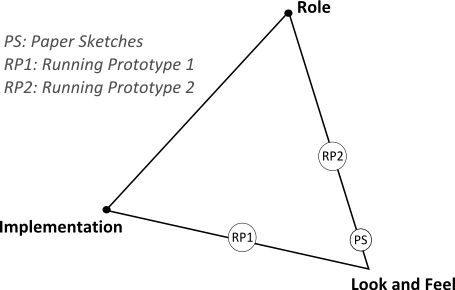
\includegraphics[width=0.7\textwidth]{hillTrianglePrototypes.png}
		\caption{\footnotesize Showing where the focus of our prototypes lie.}
		\label{fig:hillTrianglePrototypex}
\end{figure}

\section{Focus group}
We considered performing usability tests instead of focus groups to get feedback on the system. In the end we decided to conduct focus groups because the main priority was to evaluate the visualizations and not the application as a whole. Usability test focus more on navigating and completing tasks in a system, which is not the focus of this study. Focus groups are also less time consuming and gives the participants the ability to discuss different parts of the system and suggest new features and improvements. We can also use the focus groups to discuss other topics such as scenarios and requirements. Detailed information on how the first focus group was conducted and its results can be found in Chapter~\ref{ch:focusGroup1} while the second focus group is covered in Chapter~\ref{ch:focusGroup2}.

\section{Questionnaire}
A questionnaire was prepared for the second focus group. The purpose was to gain background information about the participants, and to gain an understanding of their attitude towards technology. The questionnaire also asked the participants if they thought using technology such as the one presented in the focus group would improve the quality and effectiveness of their work. The questionnaire was answered at the start of the second focus group. The information received from it is summarized in Section~\ref{sec:participants}
